\documentclass[xcolor=table,9pt]{beamer}

\usetheme{Frankfurt}
\usecolortheme{crane}
\useinnertheme{circles}

\usepackage{color, colortbl}
\usepackage{amsmath}
\usepackage{graphicx}
\usepackage{float}
\usepackage{wrapfig}
\usepackage{multicol}
\usepackage{dcolumn,array}
\usepackage{booktabs}
\usepackage{geometry}
\usepackage{caption}
\usepackage{subcaption}
\usepackage{bbm}
\usepackage{bm}
\usepackage{natbib}
\usepackage{stackengine} 
\usepackage{multirow}

\definecolor{Gray}{gray}{0.8}

\stackMath


\begin{document}
\title{Three Essays on Shrinkage Estimation and Model Selection of Linear and Nonlinear Time Series Models}   
\author{Mario Giacomazzo} 
\date{9 May 2018} 

\frame{\titlepage} 





%%%%%%%%%%%%%%%%%%%%%%%%%%%%%%%%%%%%%%%%%%%%%%%%%%%%%%%%%%%%%%%%%%%%%%%%
%% START: INTRODUCTION
%%%%%%%%%%%%%%%%%%%%%%%%%%%%%%%%%%%%%%%%%%%%%%%%%%%%%%%%%%%%%%%%%%%%%%%%
\frame{\frametitle{Overview and Motivation} 
\begin{itemize}
\item Parametric Time Series Models \\~\
\begin{itemize}
 \item Logistic Smooth Transition Autoregressive Model (LSTAR) \citep{Terasvirta1994}
 \item Threshold Autoregressive Model (TAR)  \citep{Tong1990}
 \item Autoregressive Moving Average Model (ARMA)  \citep{Box1970} \\~\
\end{itemize}
\item Model Differences \\~\
\begin{itemize}
	\item ARMA = Popularized for Weakly Stationary Time Series
	\item LSTAR and TAR = Handling Nonlinear Behavior
	\begin{itemize}
		\item Changes in Level, Dynamics, and Volatility
		\item Alternative Approach to Handling Nonstationary and Cyclical Phenomenon
		\item Useful for Clustering and Classification of Realizations
	\end{itemize}
\end{itemize}
\end{itemize}
}

\frame{\frametitle{Overview and Motivation} 
\begin{itemize}
\item Purpose \\~\
\begin{itemize}
\item Primary Goal is Forecasting
\item Economic Variables: Past Realizations Assist in Prediction \citep{Mann1943}
\item Estimation and Fitting of ARMA \citep{Durbin1960}
\item Practical Procedures Developed for Industrial Engineering \citep{Box1970}
\item Asymmetries Noticed in US Unemployment \citep{Rothman1988,Montgomery1998,Koop1999}
\end{itemize}
\end{itemize}
}

\frame{\frametitle{Overview and Motivation} 
\begin{itemize}
	\item Model Complexity \\~\
	\begin{itemize}
		\item Determined by Order Parameters
		\begin{itemize}
			\item Autoregressive (AR)
			\item Moving Average (MA)
			\item Distributed Lag (DL)
			\item Regime-specific Model Orders \\~\
		\end{itemize}
		\item Frequentist Approach: Select Based on Information Criteria or Forecasting Performance \\~\
		\item Bayesian Approach: Reversible jump Markov Chain Monte Carlo (RJMCMC) \citep{Green1995}
		\begin{itemize}
			\item AR(P) \citep{Troughton1997}
			\item TAR(P) \citep{Campbell2004,Nieto2013}
			\item STAR(P) \citep{Lopes2006}
		\end{itemize}
	\end{itemize}
\end{itemize}
}

\frame{\frametitle{Overview and Motivation} 
\begin{itemize}
	\item Model Complexity (Cont.) \\~\
	\begin{itemize}
		\item Problem
		\begin{itemize} 
			\item Difficult When Multiple Order Parameters Must Be Chosen
			\item Often Leads to Inflexible Representations
			\item Overfitting Can Still Occur \\~\
		\end{itemize}
		\item Solution 
		\begin{itemize}
			\item Intentionally Fix Orders to Be Large
			\item Restructure Time Series Model as a High Dimensional Linear Regression
			\item Apply Penalized Estimation Methods Aimed at Sparse Models
		\end{itemize}
	\end{itemize}
\end{itemize}
}

\frame{\frametitle{Introduction: Overview and Motivation} 
	\begin{center}
	\Huge \underline{Dissertation Theme} \\
	
	\huge Bayesian Automatic Estimation and Variable Selection Procedures for Flexible Subset Models
	\end{center}
}









%%%%%%%%%%%%%%%%%%%%%%%%%%%%%%%%%%%%%%%%%%%%%%%%%%%%%%%%%%%%%%%%%%%%%%%%
%% CHAPTER 2: LOGISTIC SMOOTH TRANSITION AUTOREGRESSIVE MODEL
%%%%%%%%%%%%%%%%%%%%%%%%%%%%%%%%%%%%%%%%%%%%%%%%%%%%%%%%%%%%%%%%%%%%%%%%
\frame{\frametitle{Chapter 1: LSTAR Model} 

\begin{itemize}
\item Gaussian LSTAR$(P)$ Model With 2-Regimes \\~\
\begin{itemize}
\item Given autoregressive order $P$, let $\bm{x}_t'=[y_{t-1},y_{t-2},\cdots,y_{t-P}]$, $\bm{\alpha}'=[\alpha_1,\cdots,\alpha_P]$, and $\bm{\beta}'=[\beta_1,\cdots,\beta_P]$. 

$$y_t=(\mu_\alpha+\bm{x}'_t\bm{\alpha})(1-G(z_{t}))+(\mu_\beta+\bm{x}'_{t}\bm{\beta})G(z_{t})+\epsilon_t$$

where $\epsilon_{t}\sim \textrm{ i.i.d. } N(0,\sigma^2)$ and $G(z_t): \mathbb{R}\to\mathbbm{G}\subseteq[0,1]$. \\~\

\item For LSTAR, consider transition function $G(\cdot)$ such that
$$G(z_t,\gamma^*,\delta)=\{1+\exp[-(\gamma^*/s_Z)(z_t-\delta)]\}^{-1}$$
\begin{itemize}
	\item Threshold Parameter $\delta$ Determines When Transition Occurs
	\item Slope Parameter $\gamma=\gamma^*/s_Z$ Determines the Rate of Transition
	\item As $\gamma \to \infty$, $G(z_t,\gamma^*,\delta)$ Becomes a Step Function
\end{itemize}
\end{itemize}
\end{itemize}
}

\frame{\frametitle{Chapter 1: LSTAR Model} 
\begin{itemize}
\item Prior Distributions\\~\
	\begin{itemize}
		\item TAR\citep{Geweke1993,Chen1995,Koop1999}, STAR\citep{Lubrano2000,Lopes2006,Livingston2017} \\~\
		\item $\mu_\alpha\sim \mathcal{N}(\cdot,\cdot)$ and $\mu_\beta\sim \mathcal{N}(\cdot,\cdot)$		
		\item $\sigma^2\sim\mathcal{IG}(\cdot,\cdot)$
		\item $\gamma^*\sim\mathcal{LN}(\cdot,\cdot)$
		\item  $\delta \sim \textrm{U}[q_Z(0.15),q_Z(0.85)]$ where $q_Z(\cdot)$ is the empirical quantile function
		\item Bayesian Global-Local Shrinkage Priors for $\bm{\alpha}$ and $\bm{\beta}$ 
				$$\alpha_k,\beta_k|\lambda^2_k,\lambda^2,\sigma^2 \sim N(0,\sigma^2\lambda^2\lambda^2_k)$$
		$$\lambda^2_k \sim \pi_{Local}(.) \textrm{ and  } \lambda^2 \sim \pi_{Global}(.)$$
	\begin{itemize}
		\item LASSO \citep{Park2008,Hans2009,Schmidt2013}
		\item Regime-Specific LASSO (Separate Global Tuning Parameters)
		\item Variable Selection LASSO \citep{Lykou2013}
		\item Horseshoe \citep{Carvalho2010,Makalic2016b}
	\end{itemize}
	\end{itemize}
\end{itemize}
}


\frame{\frametitle{Chapter 1: LSTAR Model} 
\begin{itemize}
\item Transition Variable\\~\
\begin{itemize}
\item Change-Point Option: $z_t=t$
\item Exogenous Option: $z_t=x_{t-d}$
\item Endogenous Option: $z_t=y_{t-d}$ (Self-Exciting)
\item Let $\bm{d}'_t=[y_{t-1},y_{t-2},\cdots,y_{t-d_{max}}]$ and $\bm{\phi}'_t=[\phi_{1},\phi_{2},\cdots,\phi_{d_{max}}]$. Reparameterize transition variable $z_t=\bm{\phi}'\bm{d}_t$. 

$$\bm{\phi}\sim Dir\bigg(\bigg[\frac{1}{d_{max}},\frac{1}{d_{max}},\cdots,\frac{1}{d_{max}}\bigg]'\bigg)$$

Now, $z_t$ is a weighted average of all considered transition variables. Because the weights are constrained to sum to $1$, the prior for $\delta$ does not require modification. \\~\

\item Advantages
\begin{itemize}
	\item Allows for a composite transition variable
	\item Estimates a more encompassing LSTAR model.
\end{itemize}
\end{itemize}
\end{itemize}
}

\frame{\frametitle{Chapter 1: LSTAR Model} 
\begin{itemize}
\item Simulation Study\\~\

 Let $\bm{d}_t=[y_{t-1},y_{t-2},y_{t-3},y_{t-4}]'$ and $\bm{\phi}'=[\phi_1,\phi_2,\phi_3,\phi_4]$. 
\begin{equation*}
	\begin{split}
		y_t&=(-0.6y_{t-3})[1-G(y_{t-1})]+(0.02+0.75y_{t-3})[G(y_{t-1})]+\epsilon_t\\
		& \textrm{where: } G(y_{t-1})=\bigg\{1+\exp\big[-120(\bm{\phi}'\bm{d}_t-0.02)\big]\bigg\}^{-1} \\
		&\textrm{ and }\epsilon_t \sim \textrm{i.i.d. }  N (0,0.02^2)\\
	\end{split}
\end{equation*}
Under  prior $\bm{\phi}\sim Dir([0.25,0.25,0.25,0.25]')$, we conduct posterior sampling for three different threshold variables $\{z_{1,t},z_{2,t},z_{3,t}\}$ defined through $\bm{\phi}$. BHS priors are used for autoregressive coefficients.
\end{itemize}
}

\frame{\frametitle{Chapter 1: LSTAR Model} 
\begin{figure}
	\centering
	\caption{Ten Random Replications}
	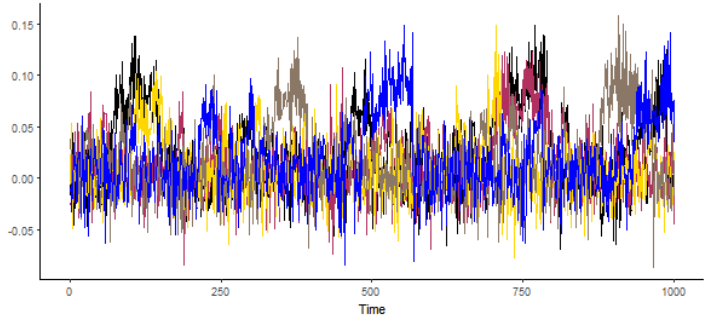
\includegraphics[scale=.42]{simplots2A}
\end{figure}
}

\frame{\frametitle{Chapter 1: LSTAR Model} 
\begin{figure}
	\centering
	\caption{Transition Function}
	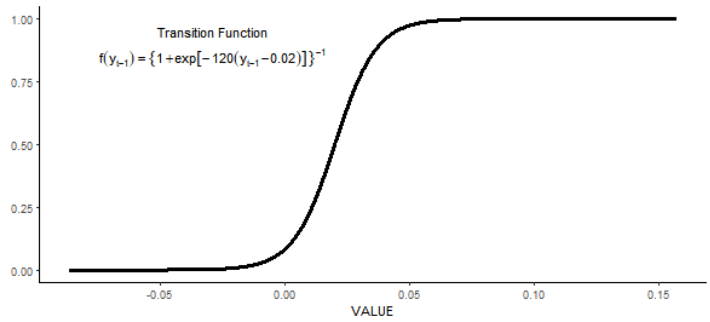
\includegraphics[scale=.42]{simplots2B}
\end{figure}
}

\frame{\frametitle{Chapter 1: LSTAR Model} 
\begin{figure}
	\centering
	\caption{Illustration of Regime-switching Behavior}
	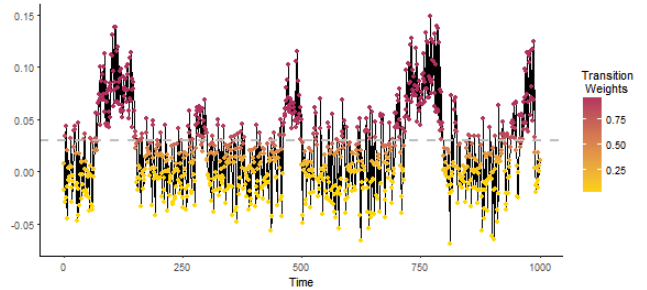
\includegraphics[scale=.5]{simplots2C}
\end{figure}
}

\frame{\frametitle{Chapter 1: LSTAR Model} 
\begin{itemize}
\item Bayesian Selection of the Threshold Variable (Scenario 1)\\~\

Consider $z_{1,t}=y_{t-1}=[1,0,0,0]\bm{d}_t$.
\begin{figure}[!h]
	\centering
	\caption{Posterior Means of $\bm{\phi}$ from 100 Replications}
      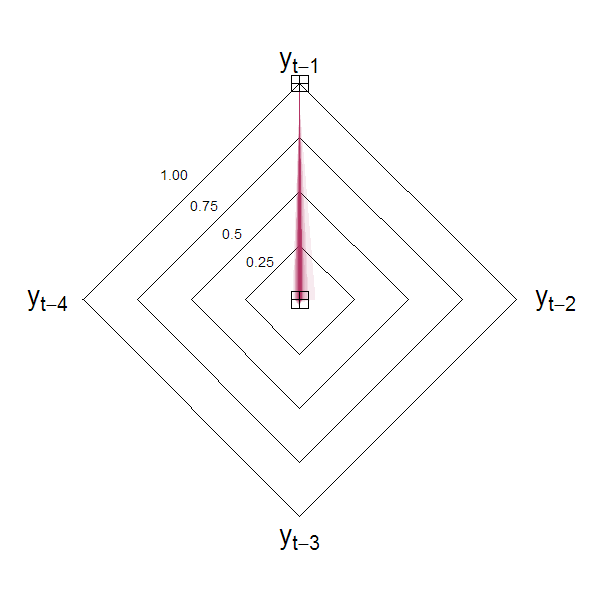
\includegraphics[scale=0.3]{hsthvar1}
\end{figure}
\end{itemize}
}

\frame{\frametitle{Chapter 1: LSTAR Model} 
\begin{itemize}
\item Bayesian Selection of the Threshold Variable (Scenario 2)\\~\

Consider  $z_{2,t}=y_{t-2}=[0,1,0,0]\bm{d}_t$.
\begin{figure}[!h]
	\centering
	\caption{Posterior Means of $\bm{\phi}$ from 100 Replications}
      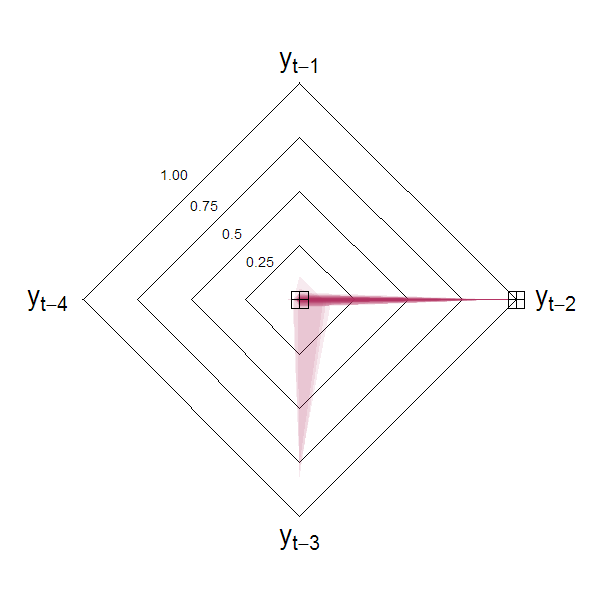
\includegraphics[scale=0.3]{hsthvar2}
\end{figure}
\end{itemize}
}

\frame{\frametitle{Chapter 1: LSTAR Model} 
\begin{itemize}
\item Bayesian Selection of the Threshold Variable (Scenario 3)\\~\

Consider  $z_{3,t}=\frac{y_{t-1}+y_{t-2}+y_{t-3}}{3}=[\frac{1}{3},\frac{1}{3},\frac{1}{3},0]\bm{d}_t$.
\begin{figure}[!h]
	\centering
	\caption{Posterior Means of $\bm{\phi}$ from 100 Replications}
      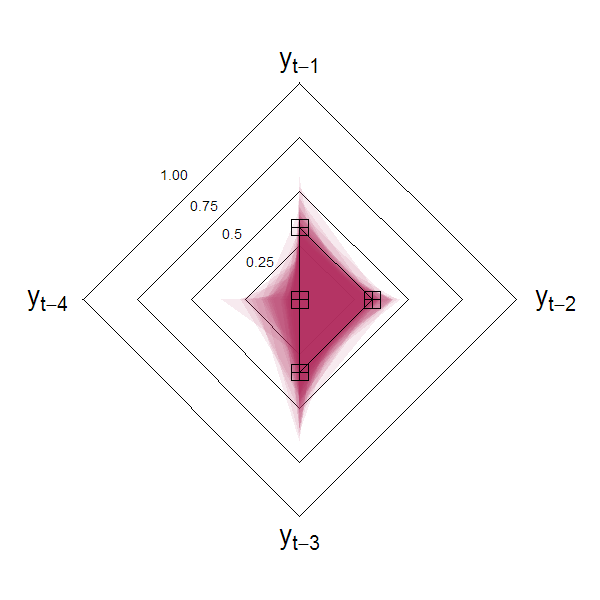
\includegraphics[scale=0.3]{hsthvar3}
\end{figure}
\end{itemize}
}

\frame{\frametitle{Chapter 1: LSTAR Model} 
\begin{itemize}
\item Application to Sunspot Data \citep{Granger1957,Terasvirta2010}\\~\
\item Application to Daily Maximum Water Temperatures \citep{Kamarianakis2016}\\~\
	\begin{itemize}
		\item Data Used From 31 Rivers in Spain
		\item Models to Forecast Daily Maximum Water Temperature
		\item Inclusion of Exogenous Distributed Lag Terms from Known Air Temperatures
		\item Horizon-Specific Models Targeting 3-step and 7-step Ahead Forecasts
		\item Nonlinear Models Improved Forecasting Accuracy for Some Rivers
	\end{itemize}
\end{itemize}
}

\frame{\frametitle{Chapter 1: LSTAR Model} 
\begin{itemize}
\item Contribution and Novelty \\~\
\begin{itemize}
	\item Efficacy of Bayesian Regularization for Nonlinear Time Series Models
	\item Use of the Dirichlet Prior Leads to More Encompassing LSTAR Specification
	\item Regime-Specific Tuning Parameters Influences Convergence in MCMC
	\item Detailed \textbf{R} Code Provided for Reproducibility \\~\
\end{itemize}
\item Feedback from \textit{International Journal of Forecasting} \\~\
\begin{itemize}
	\item Focus on Dirchlet Priors for Estimating Transition Variable
	\item Better Forecasting Application
	\item Consider Density Forecasts Along with Point Forecasts
\end{itemize}
\end{itemize}
}













%%%%%%%%%%%%%%%%%%%%%%%%%%%%%%%%%%%%%%%%%%%%%%%%%%%%%%%%%%%%%%%%%%%%%%%%
%% CHAPTER 2: THRESHOLD AUTOREGRESSIVE MODEL
%%%%%%%%%%%%%%%%%%%%%%%%%%%%%%%%%%%%%%%%%%%%%%%%%%%%%%%%%%%%%%%%%%%%%%%%


\frame{\frametitle{Chapter 2: TAR Model} 
\begin{itemize}
\item Need for Traffic Occupancy Models \\~\
	\begin{itemize}
		\item Advanced Traffic Management Systems (ATMS) Monitor Traffic Characteristics in Real Time
		\item ATMS Require Fast Short-Term Forecasting to Reduce Congestion
		\item Traffic Occupancy is the Percent of Time a Detection Zone is Occupied
		\item Different States of Traffic: Free-Flow, Congested, Transitional
		\item Factors Influencing Regime Changes : Weekly Work Patterns, Accidents, Weather, etc. \\~\
	\end{itemize}
\item Traffic Data Considered \\~\
	\begin{itemize}
		\item Major Athens' Arterial: Alexandras Ave.
		\item Time Period: April 2000
		\item Obtained by National Technical University of Athens
		\item Provided for 2013 TRANSportation Data FORecasting Competition (TRANSFOR) Developed by the Traffic Research Board (TRB) for Annual Meeting Workshop \citep{Kamarianakis2014}
		\item Measured on 90s Interval, but Mean Aggregated to 3min Interval
	\end{itemize}
\end{itemize}
}


\frame{\frametitle{Chapter 2: TAR Model} 
\begin{figure}[!h]
	\centering
	\caption{Map of Traffic Network in Athens, Greece}
      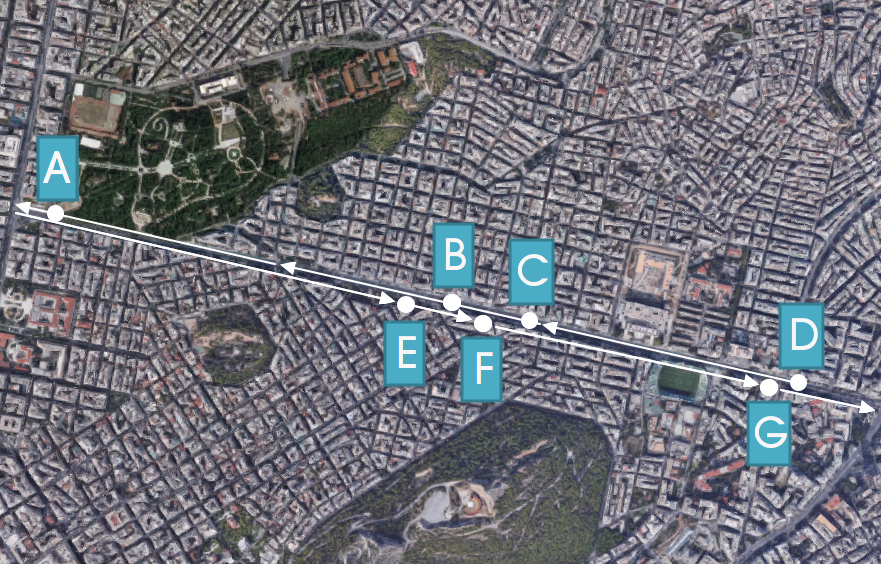
\includegraphics[scale=0.3]{TrafficMap2}
\end{figure}
}

\frame{\frametitle{Chapter 2: TAR Model} 
\begin{figure}[!h]
	\centering
	\caption{Raw Traffic Occupancy From Westbound Detectors}
      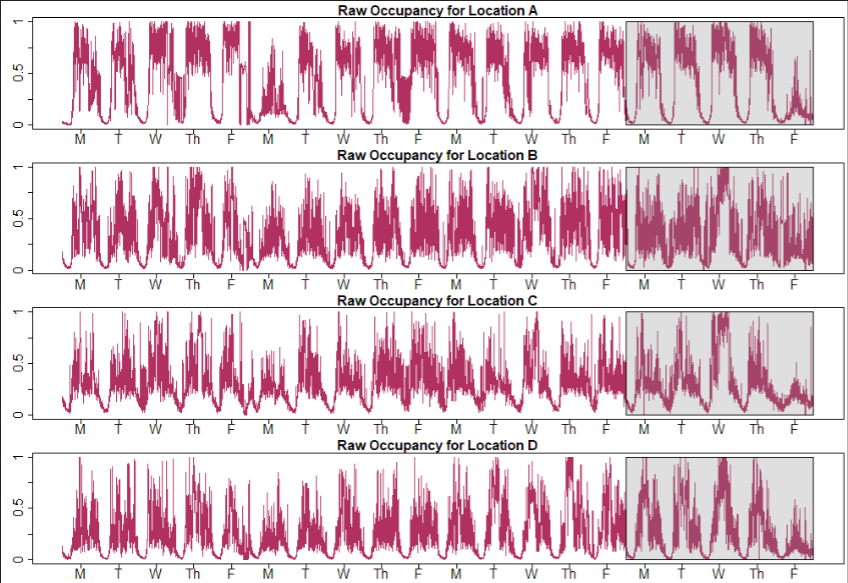
\includegraphics[scale=0.3]{RawPlotsA}
\end{figure}
}

\frame{\frametitle{Chapter 2: TAR Model} 
\begin{figure}[!h]
	\centering
	\caption{Raw Traffic Occupancy From Eastbound Detectors}
      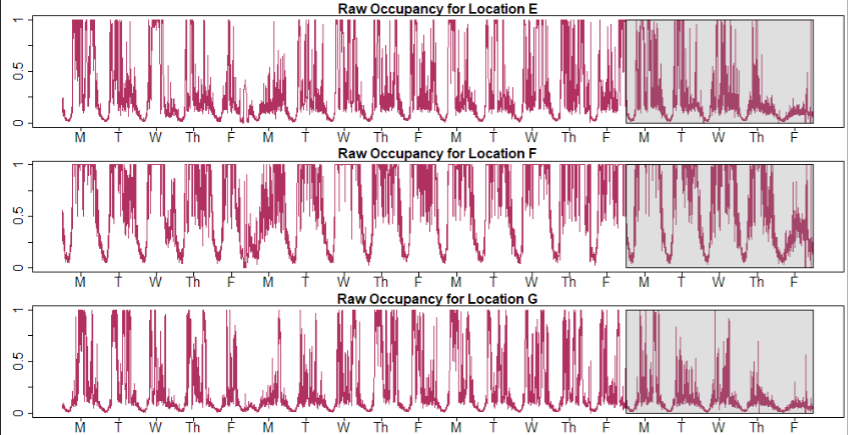
\includegraphics[scale=0.3]{RawPlotsB}
\end{figure}
}

\frame{\frametitle{Chapter 2: TAR Model} 
\begin{itemize}
\item $(L,D,h)$-Specific Models \\~\
	\begin{itemize}
		\item Location $L\in \{A,B,C,D,E,F,G\}$
		\item Work Day $D\in\{M,T,W,Th,F\}$
		\item  Horizon $h \in \{1,3,5\}$ \\~\
	\end{itemize}
\item Data Transformation \\~\
\begin{itemize}
	\item Let $O_{t}$ Represent the Traffic Occupancy at Time $t$
	\item $Y_t=\textrm{logit}(O_t)=\log[O_t/(1-O_t)]$
	\item Raw Data Adjusted at the Boundary so $\textrm{logit}(\cdot)$ Is Defined
	\item Forecasts Evaluated on Original Scale, but $$\hat{O}_{t} \neq  \textrm{logit}^{-1}(\hat{Y}_{t})$$
	\item Density Forecasts Produced from $\{\textrm{logit}^{-1}(\hat{Y}^{(s)}_{t})\}_{s=1}^{S}$ where $\{\hat{Y}^{(s)}_{t}\}_{s=1}^{S}$ are $S$ posterior samples obtained from the posterior predictive distribution $f(\hat{Y}_{t}|\mathcal{I}^*_t)$ where $\mathcal{I}^*_t=\{y_{k}\}_{k=t-h}^{t-h-P+1}$
\end{itemize}
\end{itemize}
}

\frame{\frametitle{Chapter 2: TAR Model} 
\begin{itemize}
\item Horizon-Specific Gaussian TAR$(P)$ Model with $(m+1)$-regimes
$$y_{t}=\phi_0^{(j)}+\sum\limits_{i=1}^P \phi^{(j)}_i y_{t-h-i+1}+\sigma\epsilon_{t}, \textrm{ for } \delta_{j-1}<y_{t-h}\leq \delta_{j}$$
where $\sigma>0$, $j\in\{1,2,\cdots,m+1\}$, $h\in \mathbb{N}$, and $\epsilon_t\sim \mathcal{N}(0,1)$. \\~\


Vector of Thresholds $\bm{\delta}=[\delta_1,\cdots,\delta_m]$. \\~\

Partitions the Process into $m+1$ regimes such that $-\infty=\delta_0<\delta_1\leq\delta_2\leq \cdots \leq \delta_m<\delta_{m+1}=\infty$.
\end{itemize}
}

\frame{\frametitle{Chapter 2: TAR Model} 
\begin{itemize}
\item High Dimensional Linear Representation \citep{Chan2015,Chan2017} \\~\
\begin{itemize}
\item Let $\bm{y}=[y_{1},\cdots,y_{T}]'$, $\bm{\epsilon}=[\epsilon_{1},\cdots,\epsilon_{T}]'$, and define matrix $\bm{X}$ by
$$
\bm{X}=\begin{bmatrix}
    1 & y_{1-h} & y_{1-h-1} & \dots  & y_{1-h-P+1} \\
    1 & y_{2-h} & y_{2-h-1} & \dots  & y_{2-h-P+1} \\
    \vdots & \vdots & \vdots & \ddots & \vdots \\
    1 & y_{T-h} & y_{T-h-1} & \dots  & y_{T-h-P+1}
\end{bmatrix}.
$$

Second Column of $\bm{X}$ Contains the $h$-Specific Transition Variable. \\~\

Model Matrix $\bm{X}$ Often Used in Linear AR$(P)$ Regressions.
\end{itemize}
\end{itemize}
}

\frame{\frametitle{Chapter 2: TAR Model} 
\begin{itemize}
\item High Dimensional Linear Representation (Cont.) \\~\
\begin{itemize}
\item Reorder $\bm{y}$, $\bm{\epsilon}$, and $\bm{X}$ According to Transition Variable

Sorting function $\pi(i):\{1,\cdots,T\}\to\{1,\cdots,T\}$  where $\pi(i)$ equates to the time index of the $i$th smallest element in $[y_{1-h},y_{2-h},\cdots,y_{T-h}]'$. Now, 
$$\bm{y}_R=[y_{\pi(1)+h},\cdots,y_{\pi(T)+h}]',$$ $$\bm{\epsilon}_R=[\epsilon_{\pi(1)+h},\cdots,\epsilon_{\pi(T)+h}]',$$ and 
$$
\bm{X}_1=\begin{bmatrix}
    1 & y_{\pi(1)} & y_{\pi(1)-1} & \dots  & y_{\pi(1)-P+1} \\
    1 & y_{\pi(2)} & y_{\pi(2)-1} & \dots  & y_{\pi(2)-P+1} \\
    \vdots & \vdots & \vdots & \ddots & \vdots \\
    1 & y_{\pi(T)} & y_{\pi(T)-1} & \dots  & y_{\pi(T)-P+1}
\end{bmatrix}=
\begin{bmatrix}
\bm{y}'_{\pi(1)} \\
\bm{y}'_{\pi(2)} \\
\vdots \\
\bm{y}'_{\pi(T)} \\
\end{bmatrix}
$$
\end{itemize}
\end{itemize}
}

\frame{\frametitle{Chapter 2: TAR Model} 
\begin{itemize}
\item High Dimensional Linear Representation (Cont.) \\~\
\begin{itemize}
\item Finite Set of $m$ Thresholds for an $(m+1)$-Regime TAR$(P)$ \\~\

Define the Empirical Quantile Function, $$q(.): [0,1]\to[\min\{y_{t-h}:t=1,2,\cdots,T\},\max\{y_{t-h}:t=1,2,\cdots,T\}]$$ \\~\ 

Select Sequence $\{p_k\}_{k=1}^m$ of $m$ Evenly Spaced Percentiles where $$p_{min}=p_1<\cdots<p_m=p_{max}$$ \\~\

For a Fully Saturated TAR Model Limited to $(m+1)$ Regimes, Fix \textit{a priori} $$\bm{\delta}=[q(p_{1}),q(p_2),\cdots,q(p_{m})]'$$ \\~\

\end{itemize}
\end{itemize}
}

\frame{\frametitle{Chapter 2: TAR Model} 
\begin{itemize}
\item High Dimensional Linear Representation (Cont.) \\~\
\begin{itemize}
\item Finite Set of $m$ Thresholds for an $(m+1)$-Regime TAR$(P)$ (Cont.) \\~\

For $j \in \{2,\cdots,m+1\}$, Let $k_j$ Represent the Number of Elements in $[y_{1-h},y_{2-h},\cdots,y_{T-h}]'$ Less than $q(p_{j-1})$ and Define 
$$\bm{X}_j=
\begin{bmatrix}
    0 & 0 & 0 & \dots  & 0 \\
    \vdots & \vdots & \vdots & \ddots & \vdots \\
    0 & 0 & 0 & \dots  & 0 \\
    1 & y_{\pi(k_j+1)} & y_{\pi(k_j+1)-1} & \dots  & y_{\pi(k_j+1)-P+1} \\
    \vdots & \vdots & \vdots & \ddots & \vdots \\
    1 & y_{\pi(T)} & y_{\pi(T)-1} & \dots  & y_{\pi(T)-P+1}
\end{bmatrix}=
\begin{bmatrix}
0 \\
\vdots \\
0\\
\bm{y}'_{\pi(k_j+1)} \\
\vdots \\
\bm{y}'_{\pi(T)} \\
\end{bmatrix}.
$$ \\~\

\item Fully Saturated $(m+1)$-Regime TAR$(P)$ as a Linear Regression \\~\
	$$\bm{y}_R =\bm{X}_R\bm{\theta}_R+\bm{\epsilon}_R$$
	$\bm{X}_R=[\bm{X}_1,\bm{X}_2,\cdots,\bm{X}_{m+1}]$ is a $T\times (P+1)(m+1)$ Matrix \\~\
	 
	$\bm{\theta}_R=[\bm{\theta}'_{1},\bm{\theta}'_2,\cdots,\bm{\theta}'_{m+1}]'$ is a $(P+1)(m+1) \times 1$ Vector of Grouped Reparameterized Coefficients \\~\
\end{itemize}
\end{itemize}
}

\frame{\frametitle{Chapter 2: TAR Model} 
\begin{itemize}
\item Baseline $(L,D)$-Specific Seasonal Model (Cont.) \\~\
$$y_{t}=\mu+\sum\limits_{j=1}^{H} \Big[\alpha_{j}\sin\Big(\frac{2\pi tj}{480}\Big)+\beta_{j}\cos\Big(\frac{2\pi tj}{480}\Big)\Big]+\sigma\epsilon_{t}$$
where $\sigma>0$, $H\in \mathbb{N}$, and $\epsilon_t\sim \mathcal{N}(0,1)$. \\~\

Representable as a High Dimensional Linear Regession,
 $$\bm{y}_F =\bm{X}_F\bm{\theta}_F+\bm{\epsilon}_F$$

\item Considerations for Traffic Occupancy \\~\
\begin{itemize}
	\item Maximum AR Order $P=7$
	\item Maximum Number of Thresholds $m=50$ 
	\item Set $p_{min}=0.15$ and $p_{max}=0.85$ 
	\item Saturated $51$-Regime TAR$(7)$ Model with $408$ Parameters in $\bm{\theta}_R$ \\~\
	\item Maximum Number of Sine/Cosine Pairs $H=150$
	\item Saturated Seasonal Harmonic Regression Model with $301$ Parameters in $\bm{\theta}_F$
\end{itemize}
\end{itemize}
}

\frame{\frametitle{Chapter 2: TAR Model} 
\begin{itemize}
\item Three-Step Procedure For Automatic Estimation and Selection \\~\
\begin{itemize}
\item Full Model $\bm{y}_R =\bm{X}_R\bm{\theta}_R+\bm{\epsilon}_R$ Nests $6.61\times 10^{122}$ Different $(m^*+1)$-Regime Subset TAR$(P)$ Models where $0\leq m^* \leq m$ \\~\
\item Step 1: Sparse Estimation Using Horseshoe+ Shrinkage Priors  \\~\
\begin{itemize}
\item Group LASSO Used by \cite{Chan2015}
\item $\textrm{BHS}^+$ Hierarchy for Each $\theta_i$ in $\bm{\theta}_R$ \citep{Bhadra2016}
\begin{equation*}
\begin{split}
	\theta_i|\lambda_i,\tau,\sigma^2 & \sim \mathcal{N}(0,\lambda^2_i\tau^2\sigma^2) \\
	\lambda_i &\sim \mathcal{C}^+(0,\eta_i)\\
	\eta_i & \sim \mathcal{C}^+(0,1)\\
	\tau &\sim \mathcal{C}^+(0,1)\\
\end{split}
\end{equation*}

\item Modified Hierarchy Required for Gibbs Sampling \citep{Makalic2016b} \\~\

If $\lambda_i^2|\nu_i\sim \mathcal{IG}(\frac{1}{2},\frac{1}{\nu_i})$ and $\nu_i \sim \mathcal{IG}(\frac{1}{2},1)$, then $\lambda_i^2 \sim \mathcal{C}^+(0,1)$ \citep{Wand2011}.

\end{itemize}
\end{itemize}
\end{itemize}
}

\frame{\frametitle{Chapter 2: TAR Model} 
\begin{itemize}
\item Three-Step Procedure For Sparse Estimation (Cont.) \\~\
\begin{itemize}
\item Step 2: Regime Identification \\~\
\begin{itemize}
 \item Good Starting Point Under Full Saturated Model $\mathcal{M}_R$ 
 \item Samples $\{\bm{\theta}^{(s)}_R\}_{s=1}^S$ and $\{\sigma^{(s)}\}_{s=1}^S$ from Joint Posterior Distribution
 \item Given Candidate Submodel $\mathcal{M}_\perp$, Posterior Samples $\{\bm{\theta}^{(s)}_\perp\}_{s=1}^S$ and $\{\sigma^{(s)}_\perp\}_{s=1}^S$ Obtained Via Projection
 \item Gaussian Linear Models \citep{Piironen2015b,Piironen2017}
	$$\bm{\theta}^{(s)}_\perp = (\mathbf{X}'_\perp \mathbf{X}_\perp)^{-1} \mathbf{X}'_\perp \mathbf{X}_R\bm{\theta}^{(s)}_R$$
$$\sigma^{(s)}_\perp=\sqrt{(\sigma^{(s)})^2+\frac{(\mathbf{X}_R\boldmath{\theta}^{(s)}_R-\mathbf{X}_\perp\bm{\theta}^{(s)}_\perp)'(\mathbf{X}_R\bm{\theta}^{(s)}_R-\mathbf{X}_\perp\bm{\theta}^{(s)}_\perp)}{T}}$$
\end{itemize}
\end{itemize}
\end{itemize}
}

\frame{\frametitle{Chapter 2: TAR Model} 
\begin{itemize}
\item Three-Step Procedure For Sparse Estimation (Cont.) \\~\
\begin{itemize}
\item Step 2: Regime Identification (Cont.) \\~\
\begin{itemize}
 \item Kullback-Leibler (KL) Divergence \citep{Kullback1951} Measures the Overall Discrepancy Between the Posterior Predictive Distributions $p(y_{T+1}|\mathcal{M}_R,\mathbf{y}_R,\mathbf{X}_R)$ and $p(y_{T+1}|\mathcal{M}_R,\mathbf{y}_\perp,\mathbf{X}_\perp)$
 \item KL Divergence for a Particular Sample
 $$d^{(s)}_{\perp}(\bm{\theta}^{(s)}_R,\sigma^{(s)})=\frac{1}{2}\log\Bigg(\frac{\sigma^{(s)}_\perp}{\sigma^{(s)}}\Bigg)^2$$
 \item Overall Discrepancy
 $$D(\mathcal{M}_{R}||\mathcal{M}_\perp)=\frac{1}{S}\sum\limits^S_{s=1} d^{(s)}_{\perp}(\bm{\theta}^{(s)}_R,\sigma^{(s)})$$
\end{itemize}
\end{itemize}
\end{itemize}
}

\frame{\frametitle{Chapter 2: TAR Model} 
\begin{itemize}
\item Three-Step Procedure For Sparse Estimation (Cont.) \\~\
\begin{itemize}
\item Step 2: Regime Identification (Cont.) \\~\
\begin{itemize}
 \item Forward Stepwise Selection Algorithm \citep{Peltola2014} \\~\
 
 Begin with Linear AR$(P)$ Model, Denoted $\mathcal{M}^{(1)}_\perp$, where $$\bm{\theta}^{(1)}_\perp=[\bm{\theta}'_1,\bm{0}',\bm{0}',\cdots,\bm{0}']',$$
 with initial discrepancy $D(\mathcal{M}_{R}||\mathcal{M}^{(1)}_{\perp})$ \\~\
 
  For each $j \in \{2,\cdots,m+1\}$, $\bm{\theta}_j$ is Added to $\bm{\theta}^{(1)}_\perp$ and the Best $2$-Regime TAR$(P)$ Model $\mathcal{M}^{(2)}_\perp$  Minimizes the Discrepancy $D(\mathcal{M}_{R}||\mathcal{M}^{(2)}_{\perp})$. \\~\
  
  Continue to Identify the Best $3$-Regime TAR, $4$-Regime TAR, $\cdots$ \\~\
  
  Stopping Rule Based on Relative Explanatory Power ($RelE$) from \cite{Dupuis2003}
  $$RelE(\mathcal{M}_\perp)=1-\frac{D(\mathcal{M}||\mathcal{M}_\perp)}{D(\mathcal{M}||\mathcal{M}_\perp^{(1)})}$$ \\~\
\end{itemize}
\end{itemize}
\end{itemize}
}

\frame{\frametitle{Chapter 2: TAR Model} 
\begin{itemize}
\item Three-Step Procedure For Sparse Estimation (Cont.) \\~\
\begin{itemize}
\item Step 3: Final Subset Selection \\~\
\begin{itemize}
 \item Let $\mathcal{J}=\{j: \bm{\theta}_j \neq 0\}$ indicate the AR$(P)$ parameter groups in $\bm{\theta}_R$ Selected Via Forward Algorithm
 \item Let $\theta_{i,j}$ Represent the $i$th Parameter in the $j$th Vector $\bm{\theta}_j$ for $i\in \{1,2, \cdots, P+1\}$ and $j\in \{1,2,\cdots,m+1\}$.
 \item The Set $\mathcal{I}=\{\theta_{i,j}:i=1,\cdots,P+1 \textrm{ and } j\in\mathcal{J}\}$ Contains Potentially Relevant Parameters in $\bm{\theta}_R$
 \item Repeat Forward Stepwise Algorithm Across $\mathcal{I}$. The Intercept Only Model Utilized for $\mathcal{M}^{(1)}_{\perp}$. \\~\
\end{itemize}
\item Result: Final Choice $\mathcal{M}_*$ is a $(m^*+1)$-Regime Subset TAR$(P)$ Model where $m^*$ is the Number of Parameter Groups with at Least 1 Selected Parameter. 
\end{itemize}
\end{itemize}
}

\frame{\frametitle{Chapter 2: TAR Model} 
\begin{itemize}
\item Results \\~\
\begin{itemize}
\item $(L,D)$-Specific Seasonal Profiles (Quickly Forecasts at All Horizons) 
	\begin{figure}[!h]
			\centering
			\caption{Forecasts Based on Seasonal Profiles for Westbound Detectors}
      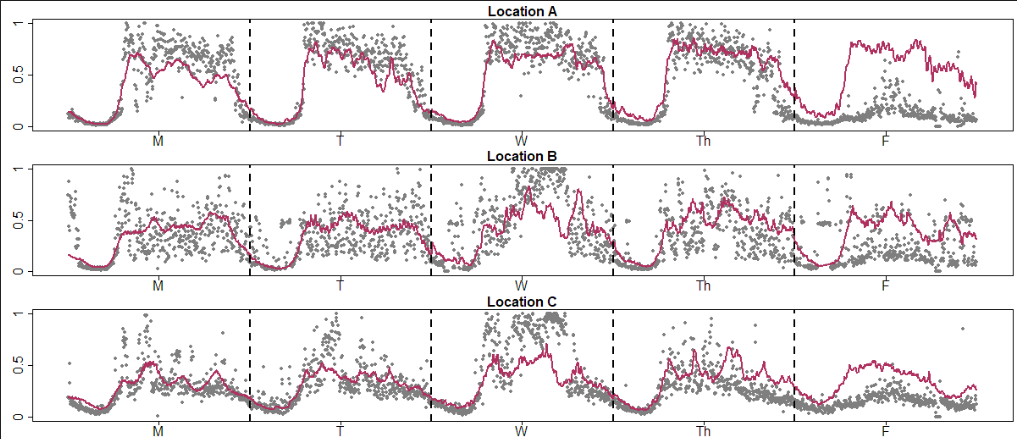
\includegraphics[scale=0.25]{SEASESTPlotsA}
	\end{figure}
\end{itemize}
\end{itemize}
}

\frame{\frametitle{Chapter 2: TAR Model} 
\begin{itemize}
\item Results (Cont.) \\~\
\begin{itemize}
\item $(L,D,1)$-Specific Final Subset TAR$(7)$ Models
	\begin{figure}[!h]
			\centering
			\caption{1-Step Ahead Density TAR Forecasts for Westbound Detectors}
      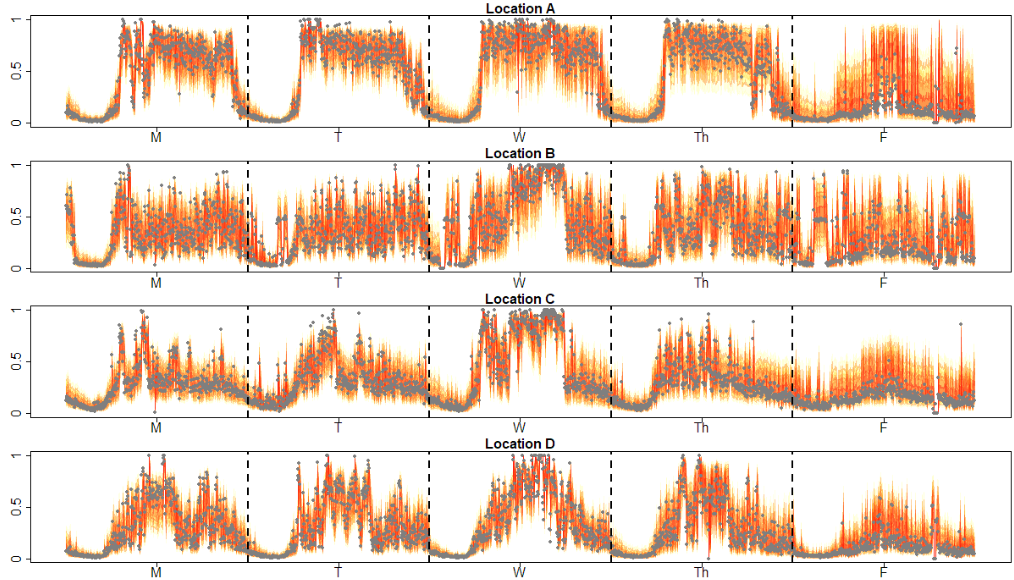
\includegraphics[scale=0.25]{DENS1PlotsA}
	\end{figure}
\end{itemize}
\end{itemize}
}

\frame{\frametitle{Chapter 2: TAR Model} 
\begin{itemize}
\item Results (Cont.) \\~\
\begin{itemize}
\item $(L,D,3)$-Specific Final Subset TAR$(7)$ Models
	\begin{figure}[!h]
			\centering
			\caption{3-Step Ahead Density TAR Forecasts for Westbound Detectors}
      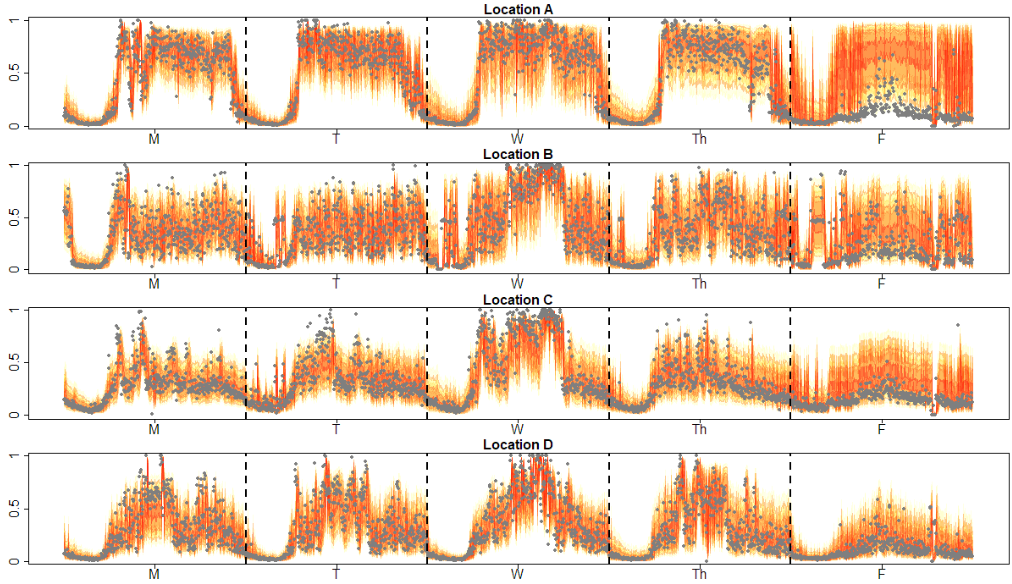
\includegraphics[scale=0.25]{DENS3PlotsA}
	\end{figure}
\end{itemize}
\end{itemize}
}

\frame{\frametitle{Chapter 2: TAR Model} 
\begin{itemize}
\item Results (Cont.) \\~\
\begin{itemize}
\item $(L,D,5)$-Specific Final Subset TAR$(7)$ Models
	\begin{figure}[!h]
			\centering
			\caption{5-Step Ahead Density TAR Forecasts for Westbound Detectors}
      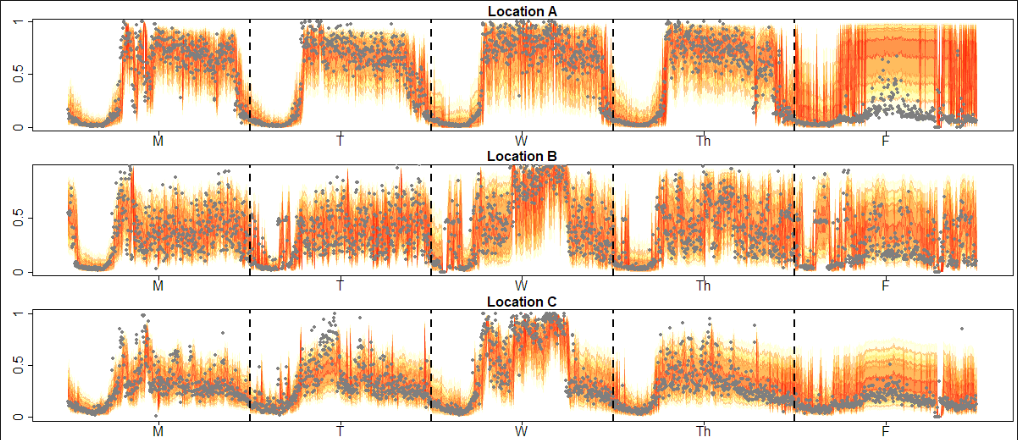
\includegraphics[scale=0.25]{DENS5PlotsA}
	\end{figure}
\end{itemize}
\end{itemize}
}

\frame{\frametitle{Chapter 2: TAR Model} 
\begin{itemize}
\item Results (Cont.) \\~\
\begin{itemize}
\item Comparison of Point Forecasts \\~\
	\begin{itemize}
	\item Evaluated on Mean Absolute Scaled Forecast Error \citep{Hyndman2006}
	$$\textrm{MASFE}(h)=\frac{1}{T_h}\sum\limits_{t=P+h}^{480}\left|\frac{O_{t}-\widehat{O}_{t}}{\textrm{MAE}_{RW}(h)}\right|$$
	\item $\textrm{MAE}_{RW}(h)$ is the Fitted MAE from Naive Random Walk where  $\widehat{O}_{t}=O_{t-h}$
	\end{itemize}

	\begin{table}[htbp]
\scriptsize
\centering
\caption{1-Step Ahead MASFE Forecast Comparison}
\begin{tabular}{c|rccccccc}
  \hline
  & & \multicolumn{7}{c}{Location}\\
  \cline{5-7}
Day & Model & A & B & C & D & E & F & G \\ 
  \hline
  \multirow{2}{*}{M} & TAR & 1.02 & 1.10 & 0.88 & 1.07 & 1.87 & 0.81 & 1.48 \\ 
  & SEAS & 1.80 & 1.47 & 1.15 & 1.43 & 4.02 & 1.57 & 3.66 \\ 
  \hline
  \multirow{2}{*}{T}  & TAR & 0.90 & 1.05 & 1.04 & 0.98 & 1.36 & 1.03 & 1.95 \\ 
  & SEAS & 1.35 & 1.36 & 1.22 & 1.46 & 3.36 & 1.65 & 3.29 \\ 
  \hline
   \multirow{2}{*}{W} & TAR & 1.04 & 1.11 & 0.91 & 0.97 & 2.27 & 1.86 & 1.55 \\ 
   & SEAS & 1.39 & 2.01 & 2.18 & 1.61 & 4.65 & 2.90 & 2.80 \\ 
  \hline
 \multirow{2}{*}{Th} & TAR & 0.93 & 0.89 & 0.82 & 0.92 & 1.48 & 1.52 & 1.83 \\ 
   & SEAS & 1.44 & 1.43 & 1.51 & 1.42 & 3.98 & 2.74 & 4.07 \\ 
  \hline
  \multirow{2}{*}{F} & TAR & 1.80 & 1.08 & 1.01 & 0.85 & 1.45 & 2.40 & 1.16 \\ 
   & SEAS & 4.77 & 2.23 & 1.98 & 1.83 & 4.37 & 6.24 & 3.78 \\ 
   \hline
\end{tabular}
\end{table}	
	
\end{itemize}
\end{itemize}
}


\frame{\frametitle{Chapter 2: TAR Model} 
\begin{itemize}
\item Results (Cont.) \\~\
\begin{itemize}
\item Comparison of Point Forecasts (Cont.) \\~\

	\begin{table}[htbp]
\scriptsize
\centering
\caption{3-Step Ahead MASFE Forecast Comparison}
\begin{tabular}{c|rccccccc}
  \hline
    & & \multicolumn{7}{c}{Location}\\
  \cline{5-7}
Day & Model & A & B & C & D & E & F & G \\ 
  \hline
  \multirow{2}{*}{M} & TAR & 0.94 & 1.06 & 0.88 & 1.13 & 1.85 & 0.88 & 1.50 \\ 
   & SEAS & 1.36 & 1.17 & 0.93 & 1.14 & 2.91 & 1.19 & 2.57 \\ 
   \hline
  \multirow{2}{*}{T} & TAR & 0.87 & 1.04 & 0.96 & 1.03 & 1.46 & 1.15 & 1.21 \\ 
   & SEAS & 1.04 & 1.06 & 0.91 & 1.10 & 2.24 & 1.22 & 2.15 \\ 
   \hline 
  \multirow{2}{*}{W} & TAR & 1.09 & 1.15 & 1.10 & 0.99 & 1.75 & 2.00 & 1.26 \\ 
   & SEAS & 1.15 & 1.61 & 1.69 & 1.21 & 2.94 & 2.24 & 1.71 \\ 
   \hline
 \multirow{2}{*}{Th}  & TAR & 0.90 & 0.96 & 0.82 & 0.93 & 1.88 & 1.47 & 1.14 \\ 
   & SEAS & 1.15 & 1.09 & 1.14 & 1.03 & 2.69 & 1.96 & 2.68 \\ 
  \hline
  \multirow{2}{*}{F} & TAR & 3.04 & 1.09 & 1.00 & 0.66 & 1.14 & 2.47 & 0.92 \\ 
   & SEAS & 3.53 & 1.57 & 1.42 & 1.33 & 3.12 & 4.35 & 2.42 \\ 
   \hline
\end{tabular}
\end{table}

\end{itemize}
\end{itemize}
}

\frame{\frametitle{Chapter 2: TAR Model} 
\begin{itemize}
\item Results (Cont.) \\~\
\begin{itemize}
\item Comparison of Point Forecasts (Cont.) \\~\

	\begin{table}[htbp]
\scriptsize
\centering
\caption{5-Step Ahead MASFE Forecast Comparison}
\begin{tabular}{c|rccccccc}
  \hline
    & & \multicolumn{7}{c}{Location}\\
  \cline{5-7}
Day & Model & A & B & C & D & E & F & G \\ 
  \hline
  \multirow{2}{*}{M} & TAR & 0.94 & 0.99 & 0.89 & 1.12 & 1.97 & 0.86 & 1.68 \\ 
   & SEAS & 1.24 & 1.06 & 0.88 & 1.06 & 2.46 & 1.08 & 2.17 \\ 
  \hline
  \multirow{2}{*}{T}  & TAR & 0.81 & 1.05 & 0.95 & 1.00 & 1.47 & 1.13 & 1.15 \\ 
   & SEAS & 0.95 & 0.95 & 0.85 & 0.99 & 1.85 & 1.07 & 1.77 \\ 
  \hline
  \multirow{2}{*}{W}  & TAR & 1.02 & 1.12 & 1.04 & 0.99 & 1.67 & 1.94 & 1.26 \\ 
   & SEAS & 1.01 & 1.44 & 1.56 & 1.12 & 2.30 & 1.95 & 1.44 \\ 
  \hline
  \multirow{2}{*}{Th}  & TAR & 0.84 & 0.98 & 0.82 & 0.87 & 1.51 & 1.48 & 1.22 \\ 
   & SEAS & 1.05 & 1.03 & 1.07 & 0.94 & 2.13 & 1.73 & 2.24 \\ 
  \hline
  \multirow{2}{*}{F}  & TAR & 2.85 & 1.20 & 0.88 & 0.70 & 1.26 & 2.52 & 1.00 \\ 
   & SEAS & 3.07 & 1.48 & 1.33 & 1.19 & 2.59 & 3.82 & 2.01 \\ 
   \hline
\end{tabular}
\end{table}

\end{itemize}
\end{itemize}
}

\frame{\frametitle{Chapter 2: TAR Model} 
\begin{itemize}
\item Contribution and Novelty \\~\
\begin{itemize}
	\item Advances Methodology for Estimating TAR$(P)$ Models with Potentially Many Regimes
	\item Shows Relevancy in an Industry Needing Short-term Forecasting
	\item Easy 3-Step Bayesian Approach Capable of Selecting  Regimes and AR Parameters Within Regimes (More Flexible Final Models)
	\item Appendix Provides Defense for Horseshoe+ Hierarchy \\~\
\end{itemize}
\item Future Developments \\~\
\begin{itemize}
	\item Modifications for Student t Distributed Errors (Shows Promise)
	\item Quality of Forecast Credible Regions
	\item Other Techniques for Modeling Heteroskedasticity
	\item Look at Using Different Transition Variables (Composite, Difference, etc.)
\end{itemize}
\end{itemize}
}















%%%%%%%%%%%%%%%%%%%%%%%%%%%%%%%%%%%%%%%%%%%%%%%%%%%%%%%%%%%%%%%%%%%%%%%%
%% CHAPTER 3: THRESHOLD AUTOREGRESSIVE MODEL
%%%%%%%%%%%%%%%%%%%%%%%%%%%%%%%%%%%%%%%%%%%%%%%%%%%%%%%%%%%%%%%%%%%%%%%%
\frame{\frametitle{Chapter 3: ARMA Model} 
\begin{itemize}
\item ARMA$(p,q)$ Model \\~\
\begin{itemize}
	\item Classic Parametric Form
	 $$\phi(B)y_t=\theta(B)\epsilon_t$$ where $$\phi(B)=1-\sum\limits_{j=1}^p \phi_j B^{j} \textrm{  and  }\theta(B)=1+\sum\limits_{k=1}^q \theta_k B^{K}$$ and $B$ Represents the Backshift Operator such that $B^ky_{t}=y_{t-k}$ \\~\
	 \item Autoregressive Order $p$ and Moving Average Order $q$
	 \item Stationary: Roots of $1-\phi_1z-\phi_2z^2-\cdots -\phi_{p}z^{p}=0$ 
	 \item Invertible: Roots of $1+\theta_1z+\theta_2z^2+\cdots +\theta_{q}z^{q}=0$ 
	 \item Multiplicative Seasonal ARMA \citep{Box1976} are Subset ARMA Processes
	 \item Presence of MA Terms Poses an Estimation Problem \citep{Hamilton1994,Cryer2008}
\end{itemize}
\end{itemize}
}

\frame{\frametitle{Chapter 3: ARMA Model} 
\begin{itemize}
\item Fast Estimation of ARMA$(p,q)$ \\~\
\begin{itemize}
	\item Residuals $\{\hat{\epsilon}_t: t=p^\prime+1,\cdots,T\}$ of a Long AR$(p^\prime)$ Process Approximate the Unobserved $\{\epsilon_t\}$ \citep{Hannan1982,Brockwell2016} \\~\
	\item Let $\bm{y}=[y_{m},\cdots,y_T]'$, $\bm{\epsilon}=[\epsilon_{m},\cdots,\epsilon_T]'$, $\bm{\beta}=[\bm{\phi}',\bm{\theta}']'=$ $[\phi_1,\cdots,\phi_p,\theta_1,\cdots,\theta_q]'$, $m=p^\prime+max\{p,q\}+1$, and 
\begin{equation*}
\bm{X}=\begin{bmatrix} \bm{x}'_{m}  \\
					\bm{x}'_{m+1}  \\
					\vdots \\
					\bm{x}'_{T} \\
	\end{bmatrix} =
	\begin{bmatrix} y_{m-1} & \cdots & y_{m-p} &
					\hat{\epsilon}_{m-1} & \cdots & \hat{\epsilon}_{m-q} \\
					y_{m} & \cdots & y_{m-p+1} &
					\hat{\epsilon}_{m} & \cdots & \hat{\epsilon}_{m-q+1} \\
					\vdots & \ddots & \vdots &\
					\vdots & \ddots & \vdots & \\
					y_{T-1} & \cdots & y_{T-p} &
					\hat{\epsilon}_{T-1} & \cdots & \hat{\epsilon}_{T-q} \\
	\end{bmatrix}.
\end{equation*}
The ARMA$(p,q)$ Model is Expressed by $\bm{y}=\bm{X}\bm{\beta}+\bm{\epsilon}$ \\~\

\item Consider $p^\prime=10\log_{10}(T)$. \cite{Hannan1984a} and \cite{Chen2011} Suggest Using Information Criteria to Select  $p^\prime$. Reduces the Loss of Data, but Substantially Effects Results.
\end{itemize}
\end{itemize}
}

\frame{\frametitle{Chapter 3: ARMA Model} 
\begin{itemize}
\item Subset ARMA$(p,q)$ Penalized Estimation Methods  \\~\
\begin{itemize}
	\item Classic Techniques \\~\
	\begin{itemize}
		\item Adaptive LASSO \citep{Zou2006}
		\begin{equation*}
\hat{\bm{\beta}}_{AL} (\lambda)= \underset{\bm{\beta}}{\textrm{argmin }}  ||\mathbf{y}-\mathbf{X}\bm{\beta}||^2 + \lambda \sum\limits_{i=1}^{p+q} \hat{w}_{i}|\beta_i|
\end{equation*}
		\item Adaptive Elastic Net \citep{Zou2009a}
		\begin{equation*}
\hat{\bm{\beta}}_{AE} (\lambda,\alpha)= \underset{\bm{\beta}}{\textrm{argmin }}  ||\mathbf{y}-\mathbf{X}\bm{\beta}||^2 + \lambda\bigg[ (1-\alpha)  \sum\limits_{i=1}^{p+q} \beta^2_i+ \alpha\sum\limits_{i=1}^{p+q} \hat{w}_{i}|\beta_i| \bigg]
\end{equation*}

		\item Vector of Weights  $\hat{\mathbf{w}}=|\hat{\bm{\beta}}_L+1/T|^{-\eta}$ where 
		\begin{equation*}
\hat{\bm{\beta}}_{L} (\lambda)= \underset{\bm{\beta}}{\textrm{argmin }}  ||\mathbf{y}-\mathbf{X}\bm{\beta}||^2 + \lambda \sum\limits_{i=1}^{p+q}|\beta_i|.
\end{equation*}
$\hat{\bm{\beta}}_{L}$ is the Original LASSO Estimate of \cite{Tibshirani1996}, and $\eta=2$, as Recommended by \cite{Zou2006,Chen2011}
	\end{itemize}

\end{itemize}
\end{itemize}
}

\frame{\frametitle{Chapter 3: ARMA Model} 
\begin{itemize}
\item Subset ARMA$(p,q)$ Penalized Estimation Methods  \\~\
\begin{itemize}
	\item Classic Techniques (Cont.) \\~\
	\begin{itemize}
		\item Optimal Selection of Tuning Parameters $\lambda$ and $\alpha$ \\~\
		
		For ADLASSO and ADENET, Model Selection Determined by $\lambda$ and $\alpha$. Two Stages Require Tuning. Estimate Prediction Error for Grid of $\lambda$ and $\alpha$  \\~\
		
		Time Series Studies Often Perform Selection Based on Out-of-Sample (OOS) Forecasting \\~\		
		
		Penalized Information Criteria Such as AIC or BIC \citep{Chen2011} \\~\
		
		Cross-Validated (CV) Measures of Error \citep{Stone1974,Hastie2009a} \\~\
		
		Appropriateness of CV Questioned in Time Series Analysis. Blocked Approaches Used for Dependent Data \citep{Burman1994, Racine2000, Arlot2010,Bergmeir2012} \\~\
		
		Regular K-Fold CV Consistently Outperforms OOS in Estimating Prediction Error \citep{Bergmeir2018}.
		
		

	\end{itemize}

\end{itemize}
\end{itemize}
}


\frame{\frametitle{Chapter 3: ARMA Model} 
\begin{itemize}
\item Subset ARMA$(p,q)$ Penalized Estimation Methods (Cont.)  \\~\
\begin{itemize}
	\item Bayesian Techniques \\~\
	\begin{itemize}
		\item Bayesian Horseshoe \citep{Carvalho2009,Carvalho2010} and Bayesian Horseshoe+ \citep{Bhadra2016} 		 Hierarchies Considered for Initial Estimation \\~\
		\item Projection Method with Forward Selection Algorithm Used to Identify the Best Model at Every Level of Flexibility from Intercept-Only to Fully Saturated ARMA$(p,q)$ \\~\
		\item Final Model Selected Based on Relative Explanatory Power ($RelE$) or Out-of-Sample Forecasting Results \citep{Piironen2017}
	\end{itemize}
\end{itemize}
\end{itemize}
}



\frame{\frametitle{Chapter 3: ARMA Model} 
\begin{itemize}
\item Overview of Methods \\~\

ADLASSO and ADENET Variants Denoted $\textrm{AL}_m$ and $\textrm{AE}_m$ where $m \in \{1,2,\cdots,11\}$

\begin{table}[htbp]
  \footnotesize
  \centering
  \caption{Summary of ADLASSO and ADENET Variants}
    \begin{tabular}{c|cc}
    \toprule
    Method ($m$) & Initial Weights (Stage 1) & Final Model (Stage 2)  \\
    \midrule
    1 & AIC & AIC\\
    2 & AIC & BIC \\
    3 & BIC & BIC \\
    \midrule
    4 & \multicolumn{2}{c}{OOS} \\
    5 & \multicolumn{2}{c}{depOOS} \\
    \midrule
    6 & \multicolumn{2}{c}{CV-5} \\
    7 & \multicolumn{2}{c}{CV-10} \\
    8 & \multicolumn{2}{c}{LOOCV} \\
    \midrule
    9 & \multicolumn{2}{c}{BCV-5} \\
    10 & \multicolumn{2}{c}{BCV-10} \\
    11 & \multicolumn{2}{c}{LOBOCV} \\
    \bottomrule
    \end{tabular}%
\end{table}%

\end{itemize}
}

\frame{\frametitle{Chapter 3: ARMA Model} 
\begin{itemize}
\item Overview of Methods (Cont.) \\~\

Bayesian Variants Denoted $\textrm{BHS}_m$ and $\textrm{BHS}^+_m$ where $m \in \{1,2,\cdots,4\}$

\begin{table}[htbp]
  \footnotesize
  \centering
  \caption{Summary of BHS and $\textrm{BHS}^+$ Variants }
    \begin{tabular}{c|cc}
    \toprule
    Method ($m$) & Final Model Selection  \\
    \midrule
    1 & $RelE(\cdot)>0.90$ \\
    2 & $RelE(\cdot)>0.95$ \\
    3 & $RelE(\cdot)>0.98$\\
    \midrule
    4 & OOS\\
    \bottomrule
    \end{tabular}%
\end{table}%

\end{itemize}
}

\frame{\frametitle{Chapter 3: ARMA Model} 
\begin{itemize}
\item Simulation Study \\~\
\begin{itemize}
\item Gaussian ARMA Processes \citep{Chen2011} \\~\
	\begin{equation*}
	y_{1,t}=0.8y_{1,t-1}+0.7y_{1,t-6}-0.56y_{1,t-7}+\epsilon_{1,t}
\end{equation*}\\~\
\begin{equation*}
	\begin{split}
	y_{2,t}&=0.8y_{2,t-1}+0.7y_{2,t-6}-0.56y_{2,t-7}\\
	&+0.8\epsilon_{2,t-1}+0.7\epsilon_{2,t-6}+0.56\epsilon_{2,t-7}+\epsilon_{2,t}
	\end{split}
\end{equation*}\\~\
\begin{equation*}
	y_{3,t}=0.8\epsilon_{3,t-1}+0.7\epsilon_{3,t-6}+0.56\epsilon_{3,t-7}+\epsilon_{3,t}
\end{equation*}\\~\

Standard Gaussian Errors $\{\epsilon_{1,t}\}$, $\{\epsilon_{2,t}\}$, and $\{\epsilon_{3,t}\}$. Abbreviated Models I, II, and III, Respectively. Samples of Length $T\in \{120, 240, 360\}$. \\~\

Data Generating Processes are Subset ARMA$(7,7)$. Maximum ARMA Orders $P=Q=14$. \\~\

\item Evaluating Subset ARMA Selection
\begin{itemize}
\item $C$: Relative Frequency of Selecting All Relevant Parameters
\item  $I$: Relative Frequency of Identifying the True Model
\item  $-$: False Negative Rate (Probability of Missing a Relevant Parameter)
\item  $+$: False Positive Rate (Probability of Selecting an Irrelevant Parameter)
\end{itemize}
\end{itemize}
\end{itemize}
}

\frame{\frametitle{Chapter 3: ARMA Model} 
\begin{itemize}
\item Simulation Study (Cont.)\\~\
\begin{itemize}
\item Sensitivity: Order Selection for Long AR$(p^\prime)$ Process

\begin{table}[htbp]
\footnotesize
\caption{Effect of Using AIC to Select $p'$ on ADLASSO Subset ARMA$(14,14)$ Estimation of Model I Based on 500 Replications}
\centering
\begin{tabular}{cc|cccc|cccc}
  \hline
  & & \multicolumn{4}{c|}{Long AR$(p')$} & \multicolumn{4}{c}{Short AR$(p')$} \\
  \cline{4-5}  \cline{8-9}
  & $T$ & $C$ & $I$ & $-$ & $+$ & $C$ & $I$ & $-$ & $+$\\
  \hline
  \multirow{3}{*}{$\textrm{AL}_1$} & 120 & 0.19 & 0.01 & 0.36 & 0.28 & 0.02 & 0.00 & 0.49 & 0.28 \\ 
  & 240 & 0.40 & 0.05 & 0.24 & 0.27 & 0.02 & 0.00 & 0.43 & 0.34 \\ 
  & 360 & 0.46 & 0.07 & 0.21 & 0.26 & 0.03 & 0.00 & 0.38 & 0.36 \\ 
  \hline
  \multirow{3}{*}{$\textrm{AL}_2$} & 120 & 0.16 & 0.04 & 0.40 & 0.17 & 0.02 & 0.00 & 0.53 & 0.18 \\ 
  & 240 & 0.36 & 0.13 & 0.27 & 0.18 & 0.01 & 0.00 & 0.47 & 0.24 \\ 
  & 360 & 0.45 & 0.17 & 0.22 & 0.18 & 0.03 & 0.01 & 0.41 & 0.27 \\ 
  \hline
  \multirow{3}{*}{$\textrm{AL}_3$} & 120 & 0.05 & 0.01 & 0.44 & 0.12 & 0.01 & 0.00 & 0.48 & 0.14 \\ 
  & 240 & 0.15 & 0.05 & 0.35 & 0.17 & 0.01 & 0.00 & 0.44 & 0.20 \\ 
  & 360 & 0.21 & 0.09 & 0.31 & 0.20 & 0.01 & 0.01 & 0.39 & 0.24 \\ 
  \hline
\end{tabular}
\end{table}

\end{itemize}
\end{itemize}
}

\frame{\frametitle{Chapter 3: ARMA Model} 
\begin{itemize}
\item Simulation Study (Cont.)\\~\
\begin{itemize}
\item Results for Model I
\end{itemize}
\begin{table}[htbp]
\footnotesize
\centering
\caption{Subset ARMA$(14,14)$ Results from 200 Replications of Model I}
\begin{tabular}{cc|cccc|cccc}
  \hline
  & & \multicolumn{4}{c|}{$\textrm{AL}_m$} & \multicolumn{4}{c}{$\textrm{AE}_m$} \\
  \cline{4-5}  \cline{8-9}
  $m$ & $T$ & $C$ & $I$ & $-$ & $+$ & $C$ & $I$ & $-$ & $+$ \\
  \hline
  1 & 360 & 0.50 & 0.08 & 0.20 & 0.24 & 0.54 & 0.08 & 0.17 & 0.25 \\ 
  2 & 360 & 0.42 & 0.16 & 0.23 & 0.19 & 0.50 & 0.20 & 0.19 & 0.15 \\ 
  3 & 360 & 0.20 & 0.10 & 0.32 & 0.19 & 0.20 & 0.10 & 0.30 & 0.19 \\
  	\hline 
  4 & 360 & 0.28 & 0.12 & 0.30 & 0.14 & 0.70 & 0.00 & 0.10 & 0.67 \\ 
  5 & 360 & 0.24 & 0.12 & 0.32 & 0.15 & 0.66 & 0.00 & 0.12 & 0.66 \\ 
  \hline
  6 & 360 & 0.36 & 0.16 & 0.27 & 0.16 & 0.52 & 0.18 & 0.19 & 0.17 \\ 
  7 & 360 & 0.44 & 0.16 & 0.23 & 0.15 & 0.54 & 0.16 & 0.18 & 0.17 \\ 
  8 & 360 & 0.42 & 0.21 & 0.24 & 0.15 & 0.53 & 0.17 & 0.19 & 0.16 \\ 
  \hline
  9 & 360 & 0.44 & 0.20 & 0.23 & 0.12 & 0.60 & 0.04 & 0.15 & 0.27 \\ 
  10 & 360 & 0.36 & 0.16 & 0.26 & 0.13 & 0.54 & 0.04 & 0.17 & 0.26 \\ 
  11 & 360 & 0.46 & 0.24 & 0.23 & 0.11 & 0.62 & 0.05 & 0.14 & 0.29 \\ 
      \hline
     & & \multicolumn{4}{c|}{$\textrm{BHS}_m$} & \multicolumn{4}{c}{$\textrm{BHS}^+_m$} \\
  \cline{4-5}  \cline{8-9}
  $m$ & $T$ & $C$ & $I$ & $-$ & $+$ & $C$ & $I$ & $-$ & $+$ \\
  \hline
  1 & 360 & 0.70 & 0.60 & 0.18 & 0.04 & 0.66 & 0.57 & 0.21 & 0.04 \\ 
  2 & 360 & 0.88 & 0.62 & 0.08 & 0.04 & 0.88 & 0.60 & 0.07 & 0.04 \\ 
  3 & 360 & 0.92 & 0.42 & 0.05 & 0.06 & 0.90 & 0.49 & 0.06 & 0.05 \\ 
  \hline
  4 & 360 & 0.92 & 0.30 & 0.04 & 0.09 & 0.92 & 0.32 & 0.05 & 0.08 \\ 
  \hline
\end{tabular}
\end{table}
\end{itemize}
}

\frame{\frametitle{Chapter 3: ARMA Model} 
\begin{itemize}
\item Simulation Study (Cont.)\\~\
\begin{itemize}
\item Results for Model II
\end{itemize}
\begin{table}[htbp]
\footnotesize
\centering
\caption{Subset ARMA$(14,14)$ Results from 200 Replications of Model II}
\begin{tabular}{cc|cccc|cccc}
  \hline
    & & \multicolumn{4}{c|}{$\textrm{AL}_m$} & \multicolumn{4}{c}{$\textrm{AE}_m$} \\
  \cline{4-5}  \cline{8-9}  
  $m$ & $T$ & $C$ & $I$ & $-$ & $+$ & $C$ & $I$ & $-$ & $+$ \\
  \hline
  1 & 360 & 0.26 & 0.01 & 0.15 & 0.38 & 0.42 & 0.00 & 0.13 & 0.38 \\ 
  2 & 360 & 0.26 & 0.02 & 0.16 & 0.32 & 0.36 & 0.02 & 0.14 & 0.33 \\ 
  3 & 360 & 0.20 & 0.01 & 0.18 & 0.30 & 0.23 & 0.02 & 0.17 & 0.31 \\ 
  \hline
  4 & 360 & 0.06 & 0.03 & 0.28 & 0.08 & 0.70 & 0.00 & 0.05 & 0.78 \\ 
  5 & 360 & 0.06 & 0.04 & 0.27 & 0.08 & 0.67 & 0.00 & 0.06 & 0.78 \\
  \hline
  6 & 360 & 0.18 & 0.05 & 0.18 & 0.25 & 0.30 & 0.00 & 0.14 & 0.32 \\ 
  7 & 360 & 0.16 & 0.04 & 0.19 & 0.24 & 0.26 & 0.01 & 0.16 & 0.30 \\ 
  8 & 360 & 0.16 & 0.02 & 0.20 & 0.26 & 0.26 & 0.01 & 0.16 & 0.31 \\ 
  \hline
  9 & 360 & 0.06 & 0.04 & 0.29 & 0.06 & 0.34 & 0.00 & 0.14 & 0.36 \\ 
  10 & 360 & 0.08 & 0.06 & 0.26 & 0.07 & 0.26 & 0.00 & 0.16 & 0.37 \\ 
  11 & 360 & 0.04 & 0.03 & 0.27 & 0.06 & 0.31 & 0.00 & 0.14 & 0.38 \\ 
    \hline
  & & \multicolumn{4}{c|}{$\textrm{BHS}_m$} & \multicolumn{4}{c}{$\textrm{BHS}^+_m$} \\
  \cline{4-5}  \cline{8-9}
  $m$ & $T$ & $C$ & $I$ & $-$ & $+$ & $C$ & $I$ & $-$ & $+$ \\
  \hline
  1 & 360 & 0.13 & 0.02 & 0.24 & 0.09 & 0.12 & 0.03 & 0.25 & 0.09 \\ 
  2 & 360 & 0.57 & 0.18 & 0.10 & 0.09 & 0.51 & 0.16 & 0.12 & 0.10 \\ 
  3 & 360 & 0.89 & 0.05 & 0.03 & 0.15 & 0.88 & 0.08 & 0.04 & 0.14 \\ 
  \hline
  4 & 360 & 0.84 & 0.09 & 0.05 & 0.17 & 0.87 & 0.10 & 0.04 & 0.15 \\ 
   \hline
\end{tabular}
\end{table}
\end{itemize}
}

\frame{\frametitle{Chapter 3: ARMA Model} 
\begin{itemize}
\item Simulation Study (Cont.)\\~\
\begin{itemize}
\item Results for Model III
\end{itemize}
\begin{table}[htbp]
\footnotesize
\centering
\caption{Subset ARMA$(14,14)$ Results from 200 Replications of Model III}
\begin{tabular}{cc|cccc|cccc}
  \hline
    & & \multicolumn{4}{c|}{$\textrm{AL}_m$} & \multicolumn{4}{c}{$\textrm{AE}_m$} \\
      \cline{4-5}  \cline{8-9}
  $m$ & $T$ & $C$ & $I$ & $-$ & $+$ & $C$ & $I$ & $-$ & $+$ \\
  \hline
  1 & 360 & 0.45 & 0.03 & 0.26 & 0.33 & 0.47 & 0.02 & 0.21 & 0.34 \\ 
  2 & 360 & 0.36 & 0.04 & 0.33 & 0.21 & 0.40 & 0.07 & 0.27 & 0.18 \\ 
  3 & 360 & 0.78 & 0.19 & 0.10 & 0.11 & 0.78 & 0.18 & 0.10 & 0.11 \\ 
  \hline
  4 & 360 & 0.49 & 0.18 & 0.24 & 0.21 & 0.86 & 0.00 & 0.05 & 0.61 \\ 
  5 & 360 & 0.52 & 0.20 & 0.23 & 0.20 & 0.90 & 0.00 & 0.03 & 0.61 \\ 
  \hline
  6 & 360 & 0.46 & 0.22 & 0.25 & 0.12 & 0.48 & 0.12 & 0.22 & 0.18 \\ 
  7 & 360 & 0.44 & 0.23 & 0.28 & 0.12 & 0.50 & 0.14 & 0.23 & 0.16 \\ 
  8 & 360 & 0.48 & 0.22 & 0.24 & 0.10 & 0.48 & 0.12 & 0.23 & 0.17 \\ 
  \hline
  9 & 360 & 0.55 & 0.14 & 0.20 & 0.15 & 0.60 & 0.04 & 0.16 & 0.29 \\ 
  10 & 360 & 0.56 & 0.21 & 0.18 & 0.14 & 0.64 & 0.02 & 0.14 & 0.25 \\ 
  11 & 360 & 0.42 & 0.08 & 0.27 & 0.19 & 0.48 & 0.01 & 0.22 & 0.34 \\ 
  \hline
    & & \multicolumn{4}{c|}{$\textrm{BHS}_m$} & \multicolumn{4}{c}{$\textrm{BHS}^+_m$} \\
  \cline{4-5}  \cline{8-9}
  $m$ & $T$ & $C$ & $I$ & $-$ & $+$ & $C$ & $I$ & $-$ & $+$ \\
  \hline
  1 & 360 & 0.26 & 0.03 & 0.46 & 0.14 & 0.26 & 0.04 & 0.46 & 0.14 \\ 
  2 & 360 & 0.40 & 0.00 & 0.34 & 0.22 & 0.38 & 0.00 & 0.36 & 0.21 \\ 
  3 & 360 & 0.62 & 0.00 & 0.18 & 0.39 & 0.59 & 0.00 & 0.20 & 0.34 \\ 
  \hline
  4 & 360 & 0.40 & 0.02 & 0.35 & 0.25 & 0.35 & 0.02 & 0.36 & 0.24 \\ 
   \hline
\end{tabular}
\end{table}
\end{itemize}
}

\frame{\frametitle{Chapter 3: ARMA Model} 
\begin{itemize}
\item Application \\~\
\begin{itemize}
	\item Monthly $\textrm{CO}_2$ Levels Measured in Mauna Loa, Hawaii \\~\
	\item Popular Textbook Example for Seasonal ARMA Processes with $Period=12$ \\~\
	\item Fitting Period: Jan 1994 - Dec 1989 (468 Time Points) \\~\
	\item Forecasting Period: Jan 1990 - Dec 1997  (96 Time Points) \\~\
	\item Apply Seasonal and Regular Differencing \\~\
\end{itemize}
\end{itemize}
}

\frame{\frametitle{Chapter 3: ARMA Model} 
\begin{itemize}
\item Application  (Cont.) 
	\begin{figure}[htbp]
	\centering
	\caption{Plots of Mauna Loa $\textrm{CO}_2$ Levels}
	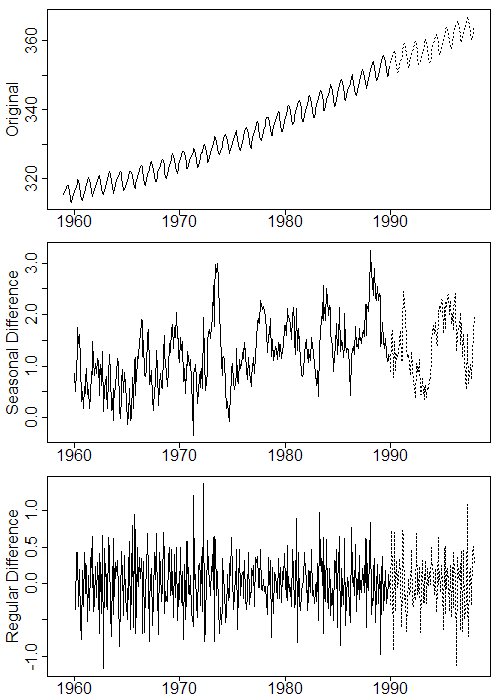
\includegraphics[scale=0.25]{co2plots}
	\end{figure}
\end{itemize}
}

\frame{\frametitle{Chapter 3: ARMA Model} 
\begin{itemize}
\item Application (Cont.) \\~\
\begin{itemize}
	\item Forecasting Metrics \\~\
	\begin{itemize}
	\item Root Mean Squared Error
	$$RMSE=\frac{1}{96} \sum\limits_{j=1}^{96} (y_j-\hat{y}_j)^2$$
	\item Mean Absolute Scaled Error
	\item Mean Bias
	$$MB=\frac{1}{96} \sum\limits_{j=1}^{96} (y_{j}-\hat{y}_{j})$$
	\item Mean Directional Bias
	$$MDB=\frac{1}{96} \sum\limits_{j=1}^{96} \textrm{sgn}(y_{j}-\hat{y}_{j})$$
	where $\textrm{sgn}(x)=1$ if $x>0$ and $\textrm{sgn}(x)=-1$ if $x<0$
	\end{itemize}
\end{itemize}
\end{itemize}
}

\frame{\frametitle{Chapter 3: ARMA Model} 
\begin{itemize}
\item Application (Cont.) 
\begin{itemize}
	\item Final Model Selection 
\end{itemize}
\begin{figure}[htbp]
	\caption{Subset ARMA Models for Mauna Loa $\textrm{CO}_2$ }
	\center
	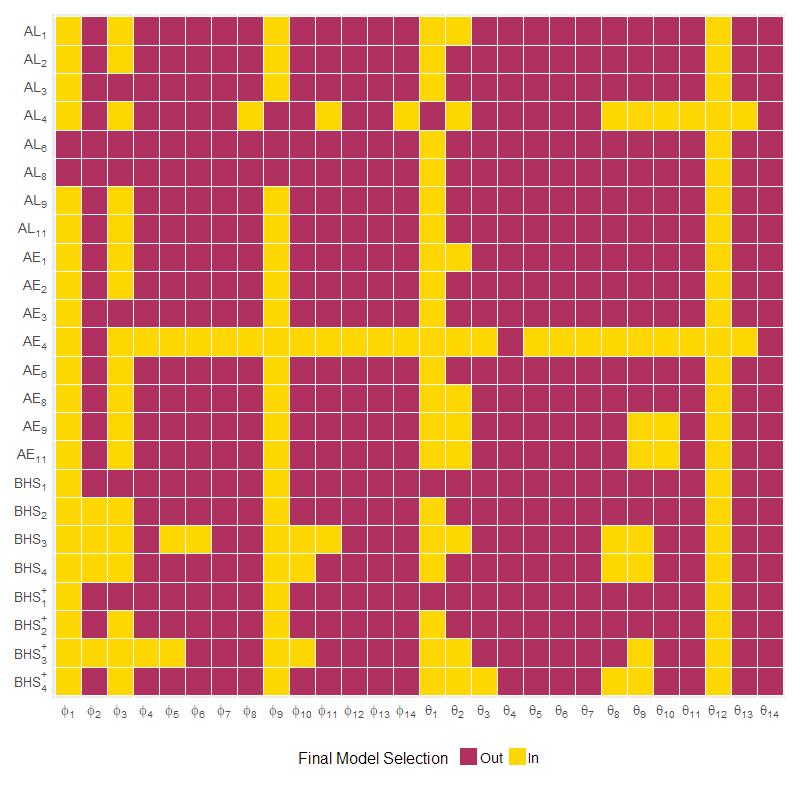
\includegraphics[scale=0.22]{maunaloaselect}
\end{figure}
\end{itemize}
}

\frame{\frametitle{Chapter 3: ARMA Model} 
\begin{itemize}
\item Application (Cont.) \\~\
\begin{itemize}
	\item Out-of-Sample Prediction
\end{itemize}
\begin{table}[htbp]
\scriptsize
\centering
\caption{One-Step Ahead Forecasting Results for Mauna Loa $\textrm{CO}_2$}
\begin{tabular}{c|cc|cc|cc|cc}
   & \multicolumn{2}{c|}{$RMSE$} & \multicolumn{2}{c|}{$MASE$} &
  \multicolumn{2}{c|}{$MB$} & \multicolumn{2}{c}{$MDB$}\\
    \hline
   m & $\textrm{AL}_m$ & $\textrm{AE}_m$ &
  $\textrm{AL}_m$ & $\textrm{AE}_m$ &
  $\textrm{AL}_m$ & $\textrm{AE}_m$ &
  $\textrm{AL}_m$ & $\textrm{AE}_m$ \\
  \hline
  1 & 0.34 & 0.34 & 0.53 & 0.53 & -0.13 & -0.13 & -0.31 & -0.29 \\ 
  2 & 0.33 & 0.33 & 0.52 & 0.52 & -0.10 & -0.10 & -0.21 & -0.21 \\ 
  3 & 0.34 & 0.34 & 0.52 & 0.52 & -0.10 & -0.10 & -0.21 & -0.21 \\ 
  4 & \multicolumn{8}{c}{Not Invertible (NI)} \\ 
  6 & 0.34 & 0.33 & 0.53 & 0.52 & -0.10 & -0.09 & -0.17 & -0.23 \\ 
  8 & 0.34 & 0.34 & 0.53 & 0.54 & -0.10 & -0.14 & -0.19 & -0.31 \\ 
  9 & 0.34 & 0.36 & 0.52 & 0.57 & -0.10 & -0.18 & -0.23 & -0.44 \\ 
  11 & 0.33 & 0.36 & 0.52 & 0.56 & -0.10 & -0.17 & -0.21 & -0.44 \\ 
  \hline
  \hline
  m & $\textrm{BHS}_m$ & $\textrm{BHS}^+_m$ &
  $\textrm{BHS}_m$ & $\textrm{BHS}^+_m$ &
  $\textrm{BHS}_m$ & $\textrm{BHS}^+_m$ &
  $\textrm{BHS}_m$ & $\textrm{BHS}^+_m$ \\
  \hline
  1 & 0.31 & 0.31 & 0.49 & 0.49 & -0.01 & -0.01 & 0.04 & 0.06 \\ 
  2 & 0.32 & 0.32 & 0.50 & 0.50 & -0.02 & -0.02 & 0.00 & -0.02 \\ 
  3 & 0.32 & 0.32 & 0.51 & 0.51 & -0.02 & -0.02 & 0.00 & 0.00 \\ 
  4 & 0.32 & 0.32 & 0.50 & 0.50 & -0.01 & -0.01 & 0.02 & 0.02 \\ 
  \hline
  \hline
  RW &  \multicolumn{2}{c|}{0.64} & \multicolumn{2}{c|}{1.03} &
  \multicolumn{2}{c|}{0.00} & \multicolumn{2}{c}{-0.02}\\
    ARMA &  \multicolumn{2}{c|}{0.37} & \multicolumn{2}{c|}{0.60} &
  \multicolumn{2}{c|}{0.01} & \multicolumn{2}{c}{0.13}\\
    SARMA &  \multicolumn{2}{c|}{0.30} & \multicolumn{2}{c|}{0.49} &
  \multicolumn{2}{c|}{-0.04} & \multicolumn{2}{c}{-0.02}\\
   \hline
\end{tabular}
\end{table}

\end{itemize}
}


\frame{\frametitle{Chapter 3: ARMA Model} 
\begin{itemize}
\item Contribution and Novelty \\~\
\begin{itemize}
	\item Highlight Issues with Previous Usage of Adaptive LASSO in Subset ARMA Selection
	\item Extends Subset ARMA Estimation to Adaptive Elastic Net 
	\item Demonstrate the Appropriateness of Multiple Cross Validation Techniques with Penalized Regression for ARMA Models
	\item Multi-step Bayesian Approach that Outperforms in Estimation, Selection, and Forecasting
	\item Provides Detailed \textbf{R} Code for Reproducibility    \\~\
\end{itemize}
\item Future Developments \\~\
\begin{itemize}
	\item Extend Theoretical Asymptotic Results for Adaptive Elastic Net
	\item More Focus on Bayesian Predictive Posterior Projection Method
	\item Consider Alternative Bayesian Handling of Moving Average Terms
\end{itemize}
\end{itemize}
}

%%%%%%%%%%%%%%%%%%%%%%%%%%%%%%%%%%%%%%%%%%%%%%%%%%%%%%%%%%%%%%%%%%%%%%%%
%% FINISH: QUESTIONS
%%%%%%%%%%%%%%%%%%%%%%%%%%%%%%%%%%%%%%%%%%%%%%%%%%%%%%%%%%%%%%%%%%%%%%%%
\frame{\frametitle{} 
	\begin{center}
	\Huge Questions?
	\end{center}
}

































































\frame[allowframebreaks]{\frametitle{References}
    {\footnotesize
    \bibliographystyle{apalike}
    \bibliography{phd}
    }
}

\end{document}

